%% LyX 2.3.7 created this file.  For more info, see http://www.lyx.org/.
%% Do not edit unless you really know what you are doing.
\documentclass[english]{article}
\usepackage{mathpazo}
\usepackage[T1]{fontenc}
\usepackage[latin9]{inputenc}
\usepackage{geometry}
\geometry{verbose,tmargin=2cm,bmargin=2cm,lmargin=2cm,rmargin=2cm}
\usepackage{amsmath}
\usepackage{amsthm}
\usepackage{amssymb}
\usepackage{graphicx}
\usepackage{setspace}

\makeatletter
%%%%%%%%%%%%%%%%%%%%%%%%%%%%%% Textclass specific LaTeX commands.
\numberwithin{equation}{section}
\numberwithin{figure}{section}

%%%%%%%%%%%%%%%%%%%%%%%%%%%%%% User specified LaTeX commands.
\usepackage{tikz}
\usetikzlibrary{external}

\makeatother

\usepackage{babel}
\begin{document}
\title{\doublespacing{}Electricity and Magnetism\linebreak{}
Tufts University\linebreak{}
Graduate School of Arts and Sciences\linebreak{}
Assignment\linebreak{}
\includegraphics{Lockups/A&S_Hori_BK+BL}}
\author{Jose Emmanuel Flores}
\date{December 1st, 2023}

\maketitle
\begin{onehalfspace}
\noindent A capacitor is made of two concentric conducting spherical
shells of radii $a$ and $b$, with $a<b$, that are maintained at
a potential difference $V_{0}$ , with the external shell being grounded.
The origin of the coordinate system is the center of the two spheres. 
\end{onehalfspace}
\begin{enumerate}
\begin{onehalfspace}
\item Using Laplace equation, find the potential for any point in the region
between the two conducting shells. Express your answer in terms of
$V_{0}$ , $a$, $b$ and the coordinates you choose. Don\textquoteright t
forget to justify your assumption. 
\item Assuming that \textbf{$b=2a$}, find the electric field in the region
between the two shells. 
\item Using general boundary conditions, find the total charge induced on
each shell. Verify your answer using Green\textquoteright s reciprocity,
and assume $b=2a$. 
\item Calculate the capacitance of this system if $a=10$ cm. Give both
the formula and the numerical value. Use the general formula $Q_{i}=C_{ij}V_{j}$
(p140 in Zangwill) and \textbf{$b=2a$}. 
\item The center of the larger sphere is now shifted by a small displacement
$\mathbf{s}$ along the z-axis: $\mathbf{s}=s\hat{\mathbf{z}}$, with
$s\ll a$. Assuming that the potential difference $V_{0}^{\prime}$
 between the two spheres is maintained constant by a battery $\left(\left|V_{0}^{\prime}\right|=\left|V_{0}\right|=\left|V_{b}-V_{a}\right|\right)$,
show that the distortion in the electric field between the conductors
created by this displacement will induce a charge on the surface of
the inner shell that is given by
\[
\sigma\left(\theta\right)=\epsilon_{0}\frac{abV_{0}}{b-a}\left[\frac{1}{a^{2}}-\frac{3s}{b^{3}-a^{3}}\cos\theta\right]
\]
\pagebreak{}
\end{onehalfspace}
\end{enumerate}
\begin{onehalfspace}
\noindent \textbf{Sol.}
\end{onehalfspace}
\begin{enumerate}
\begin{onehalfspace}
\item Laplace equation is a linear PDE, thus, the superposition principle
holds. Now, with this in mind, we can transform the problem as the
sum/superposition of the following two problems:
\end{onehalfspace}
\begin{enumerate}
\begin{onehalfspace}
\item For the inner shell, we want to find the potential outside the sphere,
assuming that the potential on the sphere is given by $V_{a}$.
\item For the outer shell, we want to find the potential inside the sphere,
assuming the potential is $V_{b}$ on the surface.
\end{onehalfspace}
\end{enumerate}
\begin{onehalfspace}
\noindent 

\noindent Now, with this in mind let's move on with the calculations.
Because we have spherical symmetry is convenient to write the Laplacian
operator in spherical coordinates, which is given by 
\[
\nabla^{2}\square=\frac{1}{r^{2}}\frac{\partial}{\partial r}\left(r^{2}\frac{\partial\square}{\partial r}\right)+\frac{1}{r^{2}\sin\theta}\frac{\partial}{\partial\theta}\left(\sin\theta\frac{\partial\square}{\partial\theta}\right)+\frac{1}{r^{2}\sin^{2}\theta}\frac{\partial^{2}\square}{\partial\varphi^{2}},
\]
now, because of the symmetry, is clear that the solution doesn't depend
on the $\varphi$ variable, i.e, we have asymuthal symmetry, and in
this case the previous operator reduces to 
\[
\nabla^{2}\square=\frac{1}{r^{2}}\frac{\partial}{\partial r}\left(r^{2}\frac{\partial\square}{\partial r}\right)+\frac{1}{r^{2}\sin\theta}\frac{\partial}{\partial\theta}\left(\sin\theta\frac{\partial\square}{\partial\theta}\right),
\]
now, the problem we want to solve is given by the following PDE $\nabla^{2}V=0$,
where $V=V\left(r,\theta\right)$, which can be written as
\[
\frac{1}{r^{2}}\frac{\partial}{\partial r}\left(r^{2}\frac{\partial V}{\partial r}\right)+\frac{1}{r^{2}\sin\theta}\frac{\partial}{\partial\theta}\left(\sin\theta\frac{\partial V}{\partial\theta}\right)=0,
\]
now, using separation or variables, we can decompose the previous
equation into to ODE, one for each variable, and then solve them separately,
which will give us the following general solution 
\begin{equation}
V\left(r,\theta\right)=\sum_{l=0}^{\infty}\left(\alpha_{l}r^{l}+\frac{\beta_{l}}{r^{l+1}}\right)P_{l}\left(\cos\theta\right),\label{eq:VGen}
\end{equation}
where $\alpha_{l},\beta_{l}$ are determined by the boundary conditions.
But this problem is even easier and instead we can use the following
argument which will simplify the previous solution: in this case the
potential will be independent of $\theta$, thus, from the PDE, we
have 
\[
\frac{1}{r^{2}}\frac{\partial}{\partial r}\left(r^{2}\frac{\partial V}{\partial r}\right)=0\implies\frac{1}{r^{2}}\frac{d}{dr}\left(r^{2}\frac{dV}{dr}\right)=0,
\]
\[
\implies\frac{d}{dr}\left(r^{2}\frac{dV}{dr}\right)=0\implies r^{2}\frac{dV}{dr}=\alpha_{1},\hspace{1em}\alpha_{1}\in\mathbb{R},
\]
then, we can integrate the previous equation as follows 
\[
\int dV=\alpha_{1}\int\frac{dr}{r^{2}}=-\frac{\alpha_{1}}{r}+\alpha_{2},\hspace{1em}\alpha_{2}\in\mathbb{R},
\]
where the $\alpha_{2}$ comes from the second integration, and then
we have 
\begin{equation}
V\left(r\right)=\alpha_{2}-\frac{\alpha_{1}}{r}.\label{eq:VGen-1}
\end{equation}
Now, the previous solution clearly doesn't have the information of
the physical problem at hand, and but we can incorpore it with the
boundary conditions, i.e, we're going to represent the $\alpha_{i}$
as functions of the known quantities. We know that the potential in
the inner shell is given by $V_{0}$, and the radius of this sphere
is $a$, thus 
\[
V_{0}=V\left(a\right)=\alpha_{2}-\frac{\alpha_{1}}{a},
\]
and on the other hand, because the exterior shell is grounded, we
have that the potential is zero, and in this case the radius is $b$,
thus 
\[
0=V\left(b\right)=\alpha_{2}-\frac{\alpha_{1}}{b}\implies\alpha_{2}=\frac{\alpha_{1}}{b},
\]
and therefore
\[
V_{0}=\frac{\alpha_{1}}{b}-\frac{\alpha_{1}}{a}=\alpha_{1}\left(\frac{1}{b}-\frac{1}{a}\right)=\alpha_{1}\left(\frac{a-b}{ab}\right)
\]
\[
\implies\alpha_{1}=\frac{ab}{a-b}V_{0},
\]
and then, the expression for the potential, in virtue of the equation
(\ref{eq:VGen-1}), is given by 
\[
V\left(r\right)=\frac{aV_{0}}{a-b}-\frac{abV_{0}}{\left(a-b\right)r},
\]
which can be simplified by 
\[
V\left(r\right)=\frac{aV_{0}}{a-b}\left(1-\frac{b}{r}\right).
\]

\end{onehalfspace}
\begin{onehalfspace}
\item For the electric field, we know that 
\[
\mathbf{E}=-\nabla V,
\]
and in this case $V$ only depends on $r$ thus 
\[
\mathbf{E}=-\frac{dV}{dr}\hat{\mathbf{r}},
\]
thus 
\[
\mathbf{E}=-\left[\frac{-abV_{0}}{\left(a-b\right)r^{2}}\right]\hat{\mathbf{r}},
\]
\[
\implies\mathbf{E}=\frac{abV_{0}}{\left(a-b\right)r^{2}}\hat{\mathbf{r}},
\]
finally, asumming $b=2a$, we have 
\[
\mathbf{E}=\frac{2a^{2}V_{0}}{ar^{2}}\hat{\mathbf{r}},
\]
\[
\therefore\mathbf{E}=\frac{2aV_{0}}{r^{2}}\hat{\mathbf{r}}.
\]
\item Now we know that 
\[
\sigma=-\epsilon_{0}\frac{\partial V}{\partial n},
\]
and from this we can calculate 
\[
Q=\int\sigma dS.
\]
And in this particular case, $\sigma$ transforms into 
\[
\sigma=-\epsilon_{0}\frac{\partial V}{\partial r},
\]
and if we assume $b=2a$, as the problem states, then 
\[
\sigma=-\epsilon_{0}\frac{2aV_{0}}{r^{2}},
\]
and from this, we have that
\end{onehalfspace}
\begin{enumerate}
\item For the inner shell 
\[
\sigma_{a}=-\epsilon_{0}\frac{2aV_{0}}{a^{2}},
\]
\[
\implies\sigma_{a}=-\epsilon_{0}\frac{2V_{0}}{a},
\]
thus, the charge will be 
\[
Q_{a}=\int-\epsilon_{0}\frac{2V_{0}}{a}dS\implies Q_{a}=-\frac{2\epsilon_{0}V_{0}}{a}\int dS,
\]
but 
\[
\int dS=4\pi r^{2},
\]
in this case $r=a$, then the total charge becomes 
\[
Q_{a}=-\frac{8\pi\epsilon_{0}V_{0}}{a}a^{2},
\]
\[
\therefore Q_{a}=-8a\pi\epsilon_{0}V_{0}.
\]
\item Now, for the exterior shell, we couls perform the same computation,
but because is grounded we don't need to do that, there's no charge
in it.
\end{enumerate}
\begin{onehalfspace}
\item Now, let's calculate the capacitance, which we know is defined by
\[
C=\frac{Q}{V_{1}-V_{2}},
\]
where the index 1 and 2 refers to thw objects in the configuration.
Then we have 
\[
C=\left.\frac{-8a\pi\epsilon_{0}V_{0}}{\frac{aV_{0}}{a-b}\left(1-\frac{b}{r}\right)}\right|_{a},
\]
but $b=2a$, then 
\[
C=\frac{-8a\pi\epsilon_{0}V_{0}}{\frac{aV_{0}}{a-2a}\left(1-\frac{2a}{a}\right)},
\]
\[
\implies C=\frac{-8a\pi\epsilon_{0}V_{0}}{-\frac{V_{0}}{2}\left(-1\right)}=16\pi a\epsilon_{0},
\]
\[
\implies C=16\pi a\epsilon_{0}.
\]
\item For this part of the problem, we have the configuration given by the
following figure:%\documentclass[border=5mm]{standalone}
%\usepackage{tikz}
%\usetikzlibrary{arrows.meta}
\begin{center}
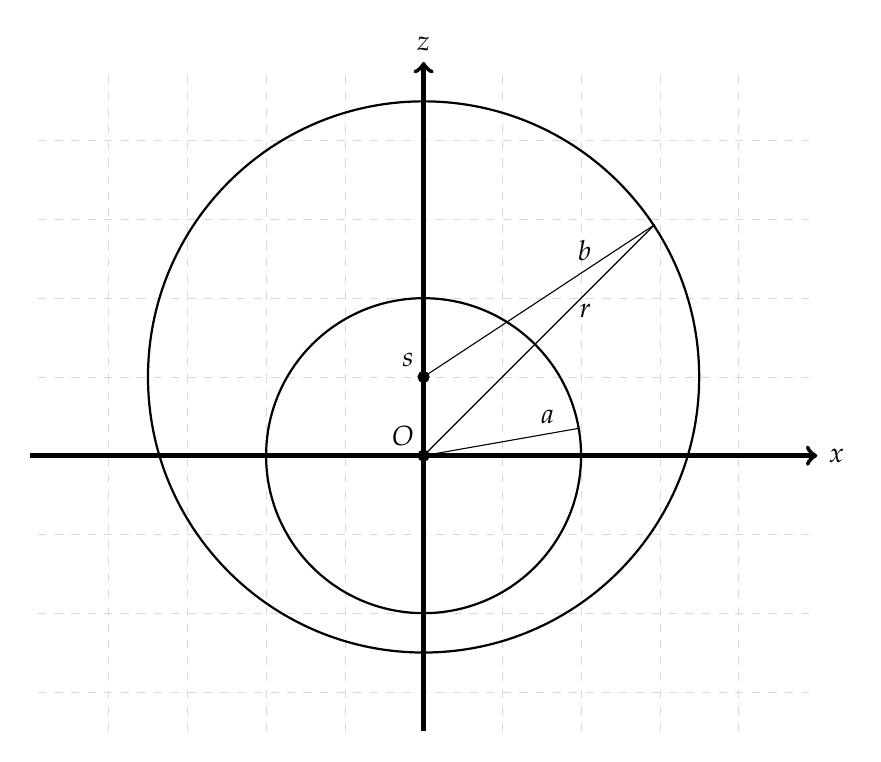
\begin{tikzpicture}

\draw[help lines, color=gray!30, dashed] (-4.9,-3.5) grid (4.9,4.9);
\draw[->,ultra thick] (-5,0)--(5,0) node[right]{$x$};
\draw[->,ultra thick] (0,-3.5)--(0,5) node[above]{$z$};

\draw [thick] circle [radius=2];
% \draw [thick] circle [radius=4];
% \draw (0,-1) circle (1.5cm);
\draw [thick] (0,1) circle [radius=3.5];

% \draw[double = gray!40, double distance=2cm, opacity=0.2] (0,0) circle (3);

\draw[-, rotate around={10:(0,0)}] (0,0) -- (2,0)  node [pos=0.8, above] {$a$};
\draw[-, rotate around={50:(0,1)}] (0,1) -- (3.35,0)  node[pos=0.7, above] {$b$};
\draw[-, rotate around={45:(0,0)}] (0,0) -- (4.15,0) node [pos=0.7, below] {$r$};
\draw[fill=black](0,0) circle (2 pt) node [anchor=south east] {$O$};
\draw[fill=black](0,1) circle (2 pt) node [anchor=south east] {$s$};

\end{tikzpicture}
\end{center}

\end{onehalfspace}

And as the problem suggest, first, we're going to prove that 
\[
r_{2}\approx b+s\cos\theta,
\]
and, in order to prove that, we are going to use the law of cosines,
which states the following 
\[
\alpha_{3}^{2}=\alpha_{1}^{2}+\alpha_{2}^{2}-2\alpha_{1}\alpha_{2}\cos\gamma,
\]
but in this case $\alpha_{1}=s$, $\alpha_{2}=r_{2}$, $\alpha_{3}=b$,
and $\gamma=\theta$, thus 
\[
b^{2}=s^{2}+r_{2}^{2}-2sr_{2}\cos\theta,
\]
but because $s\ll r_{1}$ and $r_{1}<r_{2}$, then $s\ll r_{2}$,
and this implies 
\[
b^{2}\approx r_{2}^{2}-2sr_{2}\cos\theta,
\]
and now, let's play a little bit with the math and write the rhs of
the previous equation as 
\[
b^{2}\approx r_{2}^{2}\left(1-\frac{2s}{r_{2}}\cos\theta\right),
\]
\[
\implies b\approx r_{2}\sqrt{1-\frac{2s}{r_{2}}\cos\theta},
\]
and, if we rename $x=\frac{2s}{r_{2}}\cos\theta$, we can Taylor expand
the root as follows 
\[
\sqrt{1-x}\approx1-\frac{x}{2}+\mathcal{O}\left(x^{2}\right),
\]
then, we have 
\[
b\approx r_{2}\left(1-\frac{x}{2}\right)=r_{2}\left[1-\frac{1}{2}\left(\frac{2s}{r_{2}}\cos\theta\right)\right]=r_{2}\left[1-\frac{s}{r_{2}}\cos\theta\right],
\]
\[
\implies b\approx r_{2}\left[1-\frac{s}{r_{2}}\cos\theta\right]=r_{2}-s\cos\theta,
\]
\[
\therefore r_{2}\approx b+s\cos\theta.
\]
Now, let's move to the potential part: for the inner sphere, the potential
outside goes as $1/r$, and if the spheres were concentric, then,
we know that the contribution to the total potential for the external
sphere will be constant, but a constant given by 
\[
V_{2}\sim\frac{1}{b},
\]
where $b$ is the radius of the sphere, then, using the previos result
we can state that 
\[
V_{2}\sim\frac{1}{r_{2}-s\cos\theta},
\]
and again, if we play a little bit with the math 
\[
V_{2}\sim\frac{1}{r_{2}}\frac{1}{\left(1-\frac{s}{r_{2}}\cos\theta\right)},
\]
and if we rename $x=\frac{s}{r_{2}}\cos\theta$, then we can Taylor
expand as follows 
\[
\frac{1}{1-x}\approx1+x+\mathcal{O}\left(x^{2}\right),
\]
then, 
\[
V_{2}\sim\frac{1}{r_{2}}\left(1+\frac{s}{r_{2}}\cos\theta\right).
\]
Now, let's put all the information together:
\begin{enumerate}
\item For the inner shell the potential is given by 
\[
V_{1}=c_{1}+\frac{c_{2}}{r},
\]
where $a,b$ are determined by the boundary conditions.
\item For the outer shell, the potential is given by 
\[
V_{2}=\frac{c_{3}}{r}+c_{4}\frac{s}{r^{2}}\cos\theta,
\]
but, as we can see when we add the two potentials we'll have two terms
that go as $1/r$ and therefore, we can incorporate with just one
constant. But we need two linearly independent solutions, because
the PDE that this functions satisfy is of second order, then in order
to have two solutions, we need another solution linearly independent,
and, as the problem suggest, we can see that if we use 
\[
V_{2}=c_{3}rs\cos\theta+c_{4}\frac{s}{r^{2}}\cos\theta,
\]
then we have a complete solution.
\end{enumerate}
And with this information, then, the complete solution is given by
\[
V=c_{1}+\frac{c_{2}}{r}+c_{3}rs\cos\theta+c_{4}\frac{s}{r^{2}}\cos\theta,
\]
\begin{equation}
\therefore V=c_{1}+\frac{c_{2}}{r}+s\cos\theta\left(c_{3}r+\frac{c_{4}}{r^{2}}\right).\label{eq:V}
\end{equation}
Then, the next step is to determine the constants $c_{i}$ and for
that we need, to use the boundary conditions, i.e. 
\[
V\left(r_{1},\theta\right)=V_{a},\hspace{1em}V\left(r_{2},\theta\right)=V_{b},
\]
then 
\begin{equation}
V_{a}=V\left(r_{1},\theta\right)=c_{1}+\frac{c_{2}}{a}+s\cos\theta\left(c_{3}a+\frac{c_{4}}{a^{2}}\right),\label{eq:Va}
\end{equation}
and for the other condition 
\[
V_{b}=V\left(r_{2},\theta\right)=c_{1}+\frac{c_{2}}{b+s\cos\theta}+s\cos\theta\left[c_{3}\left(b+s\cos\theta\right)+\frac{c_{4}}{\left(b+s\cos\theta\right)^{2}}\right],
\]
but, because $s\ll b$, then 
\[
V_{b}=c_{1}+\frac{c_{2}}{b+s\cos\theta}+c_{3}\left(bs\cos\theta+s^{2}\cos^{2}\theta\right)+\frac{c_{4}s\cos\theta}{\left(b+s\cos\theta\right)^{2}},
\]
\[
\implies V_{b}\approx c_{1}+\frac{c_{2}}{b+s\cos\theta}+c_{3}bs\cos\theta+\frac{c_{4}s\cos\theta}{\left(b+s\cos\theta\right)^{2}},
\]
in which I've droped the terms with $s^{2}$, and on the other hand,
we can rewrite 
\[
\frac{1}{b+s\cos\theta}=\frac{1}{b\left(1+x\right)},\hspace{1em}x=\frac{s}{b}\cos\theta,
\]
\[
\frac{1}{\left(b+s\cos\theta\right)^{2}}=\frac{1}{b^{2}\left(1+x\right)^{2}},\hspace{1em}x=\frac{s}{b}\cos\theta,
\]
and then, we can Taylor expand using 
\[
\frac{1}{1+x}\approx1-x+\mathcal{Q}\left(x^{2}\right),
\]
\[
\frac{1}{\left(1+x\right)^{2}}\approx1-2x+\mathcal{Q}\left(x^{2}\right),
\]
then, we have 
\[
\frac{1}{b\left(1+x\right)}\approx\frac{1}{b}\left(1-\frac{s}{b}\cos\theta\right),
\]
\[
\frac{1}{b^{2}\left(1+x\right)^{2}}\approx\frac{1}{b^{2}}\left(1-\frac{2s}{b}\cos\theta\right),
\]
and then, the expression for $V_{b}$ becomes 
\[
V_{b}\approx c_{1}+\frac{c_{2}}{b}\left(1-\frac{s}{b}\cos\theta\right)+c_{3}bs\cos\theta+\frac{c_{4}s\cos\theta}{b^{2}}\left(1-\frac{2s}{b}\cos\theta\right),
\]
\[
\implies V_{b}\approx c_{1}+\frac{c_{2}}{b}-c_{2}\frac{s}{b^{2}}\cos\theta+c_{3}bs\cos\theta+\frac{c_{4}s\cos\theta}{b^{2}}-2c_{4}\frac{c_{4}s^{2}\cos^{2}\theta}{b^{3}},
\]
and, again, if we drop terms with $s^{2}$ then 
\[
V_{b}\approx c_{1}+\frac{c_{2}}{b}-c_{2}\frac{s}{b^{2}}\cos\theta+c_{3}bs\cos\theta+\frac{c_{4}s\cos\theta}{b^{2}},
\]
\begin{equation}
\implies V_{b}\approx c_{1}+\frac{c_{2}}{b}+s\cos\theta\left(c_{3}b+\frac{c_{4}}{b^{2}}-\frac{c_{2}}{b^{2}}\right).\label{eq:Vb}
\end{equation}
Now, with this information we're ready to find the constants $c_{i}$,
and for that first, we need to realize that both $V_{a}$ and $V_{b}$
are constante, i.e, indepdent of $\theta$, thus in the equations
(\ref{eq:Va}) and (\ref{eq:Vb}) the terms inside the parenthesis
must vanish, ans this give us
\[
c_{3}r+\frac{c_{4}}{r^{2}}=0\implies c_{3}=-\frac{c_{4}}{a^{3}},
\]
with 
\[
c_{3}b+\frac{c_{4}}{b^{2}}-\frac{c_{2}}{b^{2}}=0\implies c_{4}-c_{2}=-c_{3}b^{3},
\]
but $c_{4}=-c_{3}a^{3}$, then 
\[
-c_{3}a^{3}-c_{2}=-c_{3}b^{3}\implies c_{2}=c_{3}\left(b^{3}-a^{3}\right),
\]
and then we have 
\begin{equation}
c_{2}=c_{3}\left(b^{3}-a^{3}\right),\hspace{1em}c_{3}=-\frac{c_{4}}{a^{3}}.\label{eq:C2-C3}
\end{equation}
Now, let's perform $V_{a}-V_{b}$
\[
V_{a}-V_{b}=c_{1}+\frac{c_{2}}{a}-\left(c_{1}+\frac{c_{2}}{b}\right),
\]
\[
\implies V_{a}-V_{b}=\frac{c_{2}}{a}-\frac{c_{2}}{b}=c_{2}\left(\frac{1}{a}-\frac{1}{b}\right),
\]
\[
\implies V_{a}-V_{b}=c_{2}\frac{b-a}{ba},
\]
\[
\therefore c_{2}=\frac{ba}{b-a}\left(V_{a}-V_{b}\right),
\]
but using the relations in the equation (\ref{eq:C2-C3}) we have
\[
\frac{ba}{b-a}\left(V_{a}-V_{b}\right)=c_{3}\left(b^{3}-a^{3}\right)\implies\frac{ba}{\left(b-a\right)\left(b^{3}-a^{3}\right)}\left(V_{a}-V_{b}\right)=c_{3},
\]
\[
\therefore c_{3}=\frac{ba}{\left(b-a\right)\left(b^{3}-a^{3}\right)}\left(V_{a}-V_{b}\right),
\]
and 
\[
\frac{ba}{\left(b-a\right)\left(b^{3}-a^{3}\right)}\left(V_{a}-V_{b}\right)=-\frac{c_{4}}{a^{3}}\implies\frac{ba^{4}}{\left(b-a\right)\left(b^{3}-a^{3}\right)}\left(V_{a}-V_{b}\right)=-c_{4},
\]
\[
\therefore c_{4}=-\frac{ba^{4}}{\left(b-a\right)\left(b^{3}-a^{3}\right)}\left(V_{a}-V_{b}\right),
\]
thus, the constants $c_{2},c_{3}$ and $c_{4}$ are given by 
\begin{equation}
c_{2}=\frac{ba\left(V_{a}-V_{b}\right)}{b-a},\hspace{1em}c_{3}=\frac{ba\left(V_{a}-V_{b}\right)}{\left(b-a\right)\left(b^{3}-a^{3}\right)},\hspace{1em}c_{4}=-\frac{ba^{4}\left(V_{a}-V_{b}\right)}{\left(b-a\right)\left(b^{3}-a^{3}\right)}\label{eq:C1-C3}
\end{equation}
And now, in order to calculate the charge on the surface of the inner
shell we know that 
\[
\sigma\left(\theta\right)=\left.-\epsilon_{0}\frac{\partial V}{\partial r}\right|_{a},
\]
then, taking the derivative with respect to $r$ to the equation (\ref{eq:V}),
we have
\[
\frac{\partial V}{\partial r}=\frac{\partial}{\partial r}\left[c_{1}+\frac{c_{2}}{r}+s\cos\theta\left(c_{3}r+\frac{c_{4}}{r^{2}}\right)\right],
\]
\[
\implies\frac{\partial V}{\partial r}=-\frac{c_{2}}{r^{2}}+c_{3}s\cos\theta-2\frac{c_{4}}{r^{3}}s\cos\theta,
\]
then 
\[
\left.\frac{\partial V}{\partial r}\right|_{a}=-\frac{c_{2}}{a^{2}}+c_{3}s\cos\theta-2\frac{c_{4}}{a^{3}}s\cos\theta,
\]
and using the expressions for the constants $c_{i}$ given in equation
(\ref{eq:C1-C3}) we have 
\[
\left.\frac{\partial V}{\partial r}\right|_{a}=-\frac{1}{a^{2}}\left[\frac{ba\left(V_{a}-V_{b}\right)}{b-a}\right]+\left[\frac{ba\left(V_{a}-V_{b}\right)}{\left(b-a\right)\left(b^{3}-a^{3}\right)}\right]s\cos\theta-\frac{2}{a^{3}}\left[-\frac{ba^{4}\left(V_{a}-V_{b}\right)}{\left(b-a\right)\left(b^{3}-a^{3}\right)}\right]s\cos\theta,
\]
\[
\implies\left.\frac{\partial V}{\partial r}\right|_{a}=-\frac{1}{a^{2}}\left[\frac{ba\left(V_{a}-V_{b}\right)}{b-a}\right]+\left[\frac{ba\left(V_{a}-V_{b}\right)}{\left(b-a\right)\left(b^{3}-a^{3}\right)}\right]s\cos\theta-2\left[-\frac{ba\left(V_{a}-V_{b}\right)}{\left(b-a\right)\left(b^{3}-a^{3}\right)}\right]s\cos\theta,
\]
\[
\implies\left.\frac{\partial V}{\partial r}\right|_{a}=-\frac{1}{a^{2}}\left[\frac{ba\left(V_{a}-V_{b}\right)}{b-a}\right]+\left\{ \left[\frac{ba\left(V_{a}-V_{b}\right)}{\left(b-a\right)\left(b^{3}-a^{3}\right)}\right]+2\left[\frac{ba\left(V_{a}-V_{b}\right)}{\left(b-a\right)\left(b^{3}-a^{3}\right)}\right]\right\} s\cos\theta,
\]
\[
\implies\left.\frac{\partial V}{\partial r}\right|_{a}=\frac{ba\left(V_{a}-V_{b}\right)}{b-a}\left[-\frac{1}{a^{2}}+\frac{3s\cos\theta}{\left(b^{3}-a^{3}\right)}\right],
\]
\[
\implies\left.\frac{\partial V}{\partial r}\right|_{a}=\frac{ba\left(V_{b}-V_{a}\right)}{b-a}\left[\frac{1}{a^{2}}-\frac{3s\cos\theta}{\left(b^{3}-a^{3}\right)}\right],
\]
and defining $V_{0}=V_{b}-V_{a}$, we have 
\[
\left.\frac{\partial V}{\partial r}\right|_{a}=-\frac{baV_{0}}{b-a}\left[\frac{1}{a^{2}}-\frac{3s\cos\theta}{\left(b^{3}-a^{3}\right)}\right],
\]
and finnaly, the charge will be given by 
\[
\sigma\left(\theta\right)=\epsilon_{0}\frac{baV_{0}}{b-a}\left[\frac{1}{a^{2}}-\frac{3s}{\left(b^{3}-a^{3}\right)}\cos\theta\right],
\]
just as we wanted to prove.
\end{enumerate}

\end{document}
